\begin{figure}
\pgfplotsset{width=\textwidth}
\centering
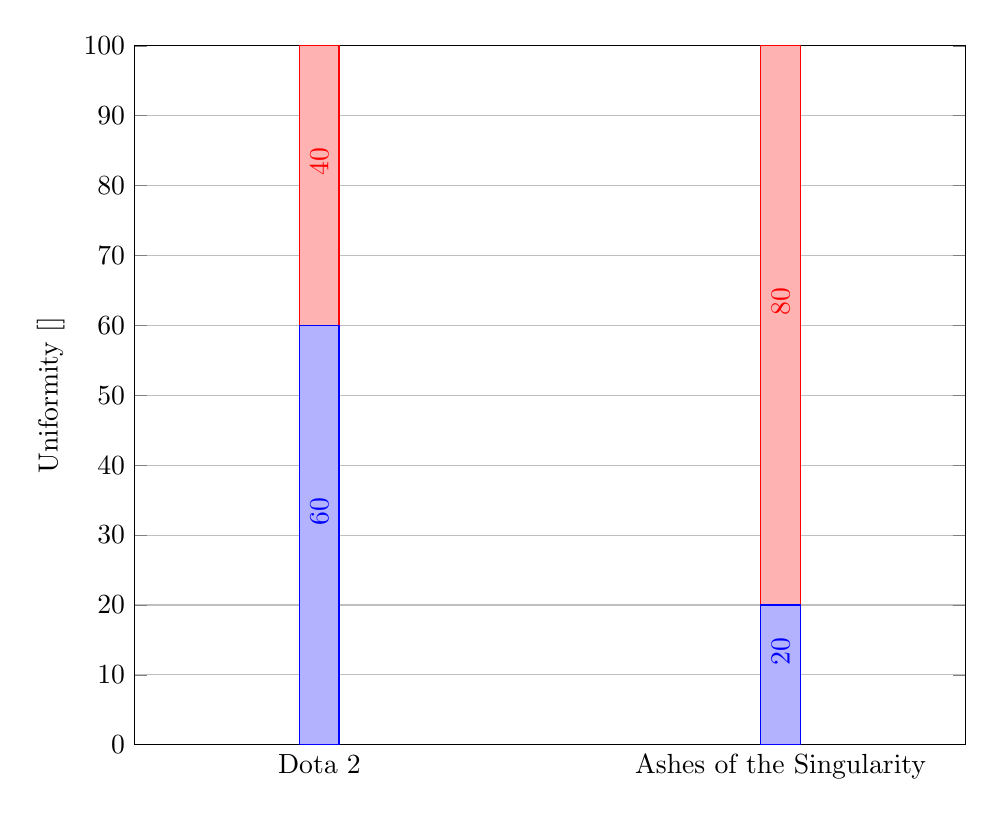
\begin{tikzpicture}
\begin{axis}[
	ybar stacked,
	enlarge x limits=0.4,
	symbolic x coords={dota,ashes},
	xticklabels={Dota 2,Ashes of the Singularity},
	xtick=data,
	ylabel={Uniformity [\SI{}{\percent}]},
	ymin=0,
	ymax=100,
	grid=both,
	nodes near coords,
	every node near coord/.append style={rotate=90, anchor=west},
	bar width=0.5cm,
	legend style={at={(1,1)},anchor=north east},
]

%\addplot [
	%fill=tumblue,
%] table[header=false] {data/registers-cs.txt};

\addplot+[ybar] plot coordinates {(dota,60) (ashes,20)};
\addplot+[ybar] plot coordinates {(dota,40) (ashes,80)};
\end{axis}
\end{tikzpicture}
\captionof{figure}{Uniformity of branches}
\label{dia:shader_by_unused}
\end{figure}
